\section{SMT Model}

\subsection{Decision Variables}

Similarly to the SAT model, the SMT model is structured based on its two tasks: \textbf{Satisfiability} and \textbf{Optimization}.

\subsubsection{Satisfiability}

The decision variables for this task are:
\begin{itemize}
    \item $match\_schedule_{p,w,m} \in \{\text{true}, \text{false}\}$: true if, and only if, the match $m \in M$ is scheduled for period $p \in P$ of week $w \in W$.
    \item $home_{p,w} = t \in T$: if t is the home team in the match in period $p \in P$ of week $w \in W$.
    \item $away_{p,w} = t \in T$: if t is the away team in the match in period $p \in P$ of week $w \in W$.
\end{itemize}

\subsubsection{Optimization}
To optimize the balance of the number of games played at home and away for each team, the following variables are utilized:
\begin{itemize}
    \item $flip\_slot_{p,w} \in \{\text{true}, \text{false}\}$: similarly to other models, it defines which team plays at home and which away in the matchup $(t_1, t_2)$ in week w and period p. If the value is false, $t_1$ plays at home, if, instead, it is true, then $t_2$ is the one playing at home.
    
    \item $homeEff_{p,w},\, awayEff_{p,w} \in T$: are, respectively, the effective home and effective away teams after the slot flip decisions.
\end{itemize}

\subsection{Objective Function}

The optimization goal is to minimize the maximum imbalance $k$ between the number of home and away games played by each team, respectively $H_t$ and $A_t$, throughout the tournament. Formally,

\[
k^* = \min \big\{\, k \mid \forall t \in T : |H_t - A_t| \leq k \big\}
\]

where:
\[
H_t = \sum_{p,w} \mathbbm{1}[\,homeEff_{p,w} = t\,], 
\quad
A_t = \sum_{p,w} \mathbbm{1}[\,awayEff_{p,w} = t\,].
\]
The effective home and away variables are computed by considering slot flips:

\begin{align*}
homeEff_{p,w} =& \text{ite}(flip\_slot_{p,w},\, away_{p,w},\, home_{p,w}), \\
awayEff_{p,w} =& \text{ite}(flip\_slot_{p,w},\, home_{p,w},\, away_{p,w}).
\end{align*}
where ite stands for "if then else" statement.

\subsection{Constraints}

\subsubsection{Each match is assigned to a unique period each week}

Each period in each week is assigned to exactly one match:

\[
\forall p \in P,\, w \in W: 
\sum_{m \in M} match\_schedule_{p,w,m} = 1.
\]
Each match is assigned to exactly one period each week:

\[
\forall m \in M,\, w \in W: 
\sum_{p \in P} match\_schedule_{p,w,m} = 1.
\]

\subsubsection{Binding team assignments}
The teams playing in the scheduled matches in $match\_schedule$ are linked to the corresponding variables $home$ and $away$ based on the values of $rb$ as follows:

\[
\forall p \in P,\, w \in W: 
\bigvee_{m \in M} \big(
match\_schedule_{p,w,m} \wedge home_{p,w} = rb_{m,w,0} \wedge away_{p,w} = rb_{m,w,1}
\big).
\]

\subsubsection{Every team plays at most twice in the same period}

For each team $t$ and each period $p$, we count how many times $t$ appears either as home or away in that period over all weeks and constraint the count to not exceed 2:

\[
\forall t \in T,\, p \in P: 
\sum_{w \in W} \sum_{m \in M} 
\big(
[\,rb_{m,w,0} = t \lor rb_{m,w,1} = t\,] \cdot [\,match\_schedule_{p,w,m}\,]
\big) \leq 2.
\]

\subsubsection{Symmetry breaking}

To reduce equivalent permutations of the solutions, the first match is fixed:

\[
match\_schedule_{0,0,0} = \text{true}.
\]

\subsection{Validation}

\subsubsection{Experimental Design}
We encode both the satisfiability and optimization phases in QF\_LIA (quantifier-free linear integer arithmetic) because it lets us combine Boolean decisions with integer sums and comparisons directly, avoiding complex encodings of counters in pure SAT.

Solver performance is measured in two stages:
\begin{enumerate}
  \item \textbf{Satisfiability}: Produce a single \texttt{.smt2} file that encodes match assignments, period-limit constraints, and symmetry breaking as linear arithmetic formulas. The solver then finds an initial feasible schedule.
  \item \textbf{Optimization}: Calculate the initial imbalance, then perform a binary search over 
  \[
    k \in \{1,2,\dots,\lfloor(N-1)/2\rfloor\}.
  \]
  For each candidate \(k\), generate a new \texttt{.smt2} file that
  \begin{itemize}
    \item reuses the base \(home/away\) assignments,
    \item adds Boolean \texttt{flip\_slot} variables,
    \item defines effective \(homeEff,awayEff\) via \texttt{ite},
    \item asserts \(\lvert H_t - A_t\rvert \le k\) using integer counters \(H_t,A_t\).
  \end{itemize}
  This produces roughly \(\log_2 N\) optimization files.
\end{enumerate}

Each file is solved with a separate \texttt{subprocess.run} call to Z3 or CVC5, and we record the wall-clock time of each invocation. The “total runtime” in Table~\ref{table:smt-result} is the sum of all individual call durations, from the first satisfiability invocation through the last optimization call, without resetting the timer. A global 300 s timeout governs both phases.


\subsubsection{Experimental results}

The experimental results show that Z3 performs significantly better than CVC5 in terms of solving time and scalability. Specifically, Z3 solved instances up to $N=22$ within the time limit, while CVC5 handled only smaller instances and degraded rapidly beyond $N=8$.

\begin{table}[H]
\centering
\small
\begin{tabular}{|c|c|c|}
\toprule
\textbf{N} & \textbf{Z3} & \textbf{CVC5} \\
\midrule
6  & \textbf{0}   & \textbf{0}   \\
8  & \textbf{0}   & \textbf{1}   \\
10 & \textbf{0}   & N/A \\
12 & \textbf{0}   & N/A \\
14 & \textbf{0}   & N/A \\
16 & \textbf{0}   & N/A \\
18 & \textbf{3}   & N/A \\
20 & \textbf{14}  & N/A \\
22 & \textbf{280} & N/A \\
24 & N/A & N/A \\
\bottomrule
\end{tabular}
\caption{SMT solver runtimes (in seconds)}
\label{table:smt-result}
\end{table}

% \begin{figure}[H]
% \centering
% 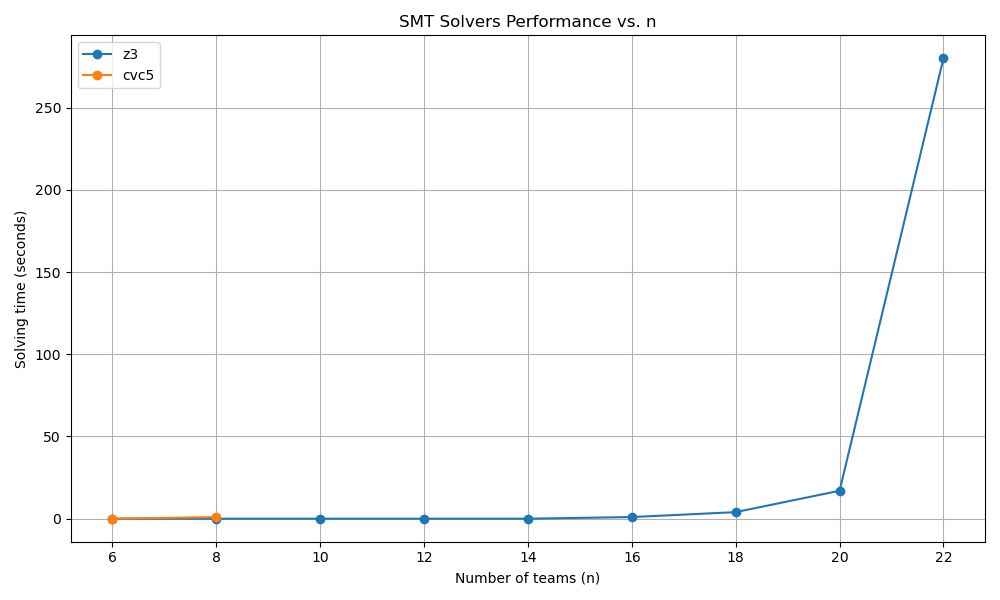
\includegraphics[width=0.8\linewidth]{img/SMT-result.png}
% \caption{SMT solution example}
% \label{fig:smt-result}
% \end{figure}
